\documentclass[12pt]{article}

\usepackage[margin=1in,footskip=0.25in]{geometry}
\usepackage{amsmath}
\usepackage{amssymb}
\usepackage{graphicx}
\usepackage{makeidx}

\makeindex

\begin{document}

\title{Fluid Mechanics for Ocean Scientists}
\author{Milan Curcic}
\date{}

\maketitle

\tableofcontents

\newpage
\section{Introduction}

\subsection{What will you learn in this course}

The course aims to provide students with a solid understanding of fluid
mechanics fundamentals relevant to ocean physics researchers.
By the end of the course, you will be proficient in applying fluid mechanical
concepts and mathematical tools to solve ocean physics research problems.
The course schedule covers a wide range of topics, starting with a review of
vector calculus and progressing through fluid kinematics, velocity gradients,
strain rates, rotation, and stress. It also includes the conservation of
volume, mass, and momentum, as well as stream functions, velocity potentials,
and Bernoulli's principle. Advanced topics such as vorticity, boundary layers,
turbulence, steady Navier-Stokes equations, flow instabilities, rotating and
stratified flows, and both surface and internal gravity waves are also covered.
The course concludes with a review and discussion session.

\subsection{Reference textbooks}

These lecture notes are based on the following textbooks:

\begin{enumerate}
  \item \textit{Fluid Mechanics}, 6th Ed., by Kundu, Cohen, and Dowling
  \item \textit{Essentials of Atmospheric and Oceanic Dynamics} by Geoffrey Vallis
\end{enumerate}

While the notes contain the distilled and required information for you to
succeed in this course, please refer to these textbooks for more detailed
explanations and examples.

\newpage
\section{Review of vector calculus}

In this section we will review the necessary concepts from vector calculus that
we will use in this course.
These include:
scalars, vectors and tensors;
gradient, divergence, and curl;
line, surface, and volume integrals;
and the Gauss and Stokes theorems.

\subsection{Scalars, vectors, and tensors}

In this course we will mainly use three types of quantities to describe fluid
properties: \textit{scalars}, \textit{vectors}, and \textit{tensors}.

\textit{Scalars}\index{Scalar} are completely described by their magnitude.
Examples of scalars are temperature, pressure, or density.
A value of 290 K, for example, completely describes the temperature of a fluid
at some point in space and time.
We will write them in equations using italics, e.g. $T$, $p$, $\rho$.

\textit{Vectors}\index{Vector} have both magnitude and direction.
Examples of vector are velocity, acceleration, or force.
In 3-dimensional Cartesian space with coordinates $(x, y, z)$, for example,
vector $\mathbf{u}(x,y,z)$ can be described by its components

\begin{equation}
  \mathbf{u} =
  \begin{bmatrix}
    u_x \\
    u_y \\
    u_z
  \end{bmatrix}
\end{equation}
where $u_x$, $u_y$, and $u_z$ (each a scalar) are the components of $\mathbf{u}$
in the $x$, $y$, and $z$ directions, respectively.
This is the conventional notation, however, we will often write vectors
inline as $\mathbf{u} = (u_x, u_y, u_z)$.
We will write vectors in equations using boldface, e.g. $\mathbf{u}$,
$\mathbf{a}$, or $\mathbf{F}$.

The magnitude\index{Vector!magnitude}, or norm\index{Vector!norm}, of a 
$\mathbf{u}$ is denoted by $||\mathbf{u}||$, and is calculated as

\begin{equation}
  ||\mathbf{u}|| = \sqrt{u_x^2 + u_y^2 + u_z^2}
\end{equation}

\textit{Tensors}\index{Tensor} have magnitude, direction, and orientation, such as stress or
strain.
They are vectors that act on each respective surface orthogonal to the direction
of the tensor.
In 3-dimensional space, for example, a stress tensor can be described as:

\begin{equation}
  \mathbf{\tau} =
  \begin{bmatrix}
    \tau_{xx} & \tau_{xy} & \tau_{xz} \\
    \tau_{yx} & \tau_{yy} & \tau_{yz} \\
    \tau_{zx} & \tau_{zy} & \tau_{zz}
  \end{bmatrix}
\end{equation}

It may be useful to think of scalars as 0$^{th}$-order tensors, vectors as
1$^{st}$-order tensors, and tensors as 2$^{nd}$-order tensors.\\

\noindent\textbf{Exercise:} Pick your favorite programming language
(or ask for a recommendation for one).
Write a program that defines a scalar, a vector, and a tensor, and assign
numerical values to them.
Print the values to the screen.
Is there a difference in how you define them in your program?\\

\subsection{Unit vectors}

Unit vectors\index{Vector!unit} are vectors with magnitude of 1.
A popular notation for unit vectors in Cartesian coordinates is $\mathbf{i}$,
$\mathbf{j}$, and $\mathbf{k}$, which point in the $x$, $y$, and $z$ directions,
respectively.
So, a vector $\mathbf{u}$ can be written as

\begin{equation}
  \mathbf{u} = u_x \mathbf{i} + u_y \mathbf{j} + u_z \mathbf{k}
\end{equation}

Notice that you can get get the unit vector by dividing any vector by its
magnitude, i.e. $\mathbf{u}/||u||$.

\subsection{Vector operations}

Two vectors can be added, subtracted, or multiplied.
Although vector addition and subtraction are straightforward, vector
multiplication is more interesting.
There are two types of vector multiplication: the \textit{dot product} and the
\textit{cross product}.

\subsubsection{Dot product}

The dot product\index{Product!dot} of two 3-dimensional Cartesian vectors
$\mathbf{a}$ and $\mathbf{b}$ is an element-wise sum of their components
(and thus, a scalar!):

\begin{equation}
  \mathbf{a} \cdot \mathbf{b} =
  \begin{bmatrix}
    a_1 \\
    a_2 \\
    a_3
  \end{bmatrix}
  \cdot
  \begin{bmatrix}
    b_1 \\
    b_2 \\
    b_3
  \end{bmatrix}
  = a_1 b_1 + a_2 b_2 + a_3 b_3
\end{equation}

More generally, the dot product of two n-dimensional vectors $\mathbf{a}$ and
$\mathbf{b}$ is

\begin{equation}
  \mathbf{a} \cdot \mathbf{b} = \sum_{i=1}^{n} a_i b_i = a_1 b_1 + a_2 b_2 + \ldots + a_n b_n
\end{equation}

The dot product is commutative, meaning that
$\mathbf{a} \cdot \mathbf{b} = \mathbf{b} \cdot \mathbf{a}$.

The magnitude of a dot product of two vectors is equal to the product of their
magnitudes and the cosine of the angle $\theta$ between them:

\begin{equation}
  \mathbf{a} \cdot \mathbf{b} = ||\mathbf{a}|| ||\mathbf{b}|| \cos{\theta}
\end{equation}
To visualize this relationship, take one vector and project it onto the other.
This projection is the magnitude of the vector times the cosine of the angle
between them.
Now one vector and the projection of the other onto the first vector are
pointing in the same direction, so their dot product is the product of their
magnitudes.
It can be useful to think of a dot product as collapsing the two vectors into a
single number contains contributions from each of their components.\\

\noindent\textbf{Exercise:} Write a program that calculates the dot product of
two vectors.\\

\noindent\textbf{Exercise:} What is the dot product of two orthogonal vectors?
How about the dot product of a vector with itself?\\

\subsubsection{Cross product}

The cross product\index{Product!cross} of two vectors $\mathbf{a}$ and
$\mathbf{b}$ is defined as:

\begin{equation}
  \mathbf{a} \times \mathbf{b} =
  det \begin{bmatrix}
    a_x & a_y & a_z \\
    b_x & b_y & b_z \\
    \mathbf{i} & \mathbf{j} & \mathbf{k}
  \end{bmatrix}
\end{equation}
where $det(\mathbf{M})$ means the \textit{determinant of matrix $\mathbf{M}$}.

Using the so-called \textit{rule of Saurus}, the cross product can be calculated
as:

\begin{equation}
  \mathbf{a} \times \mathbf{b} = (a_y b_z - a_z b_y) \mathbf{i} +
    (a_z b_x - a_x b_z) \mathbf{j} + (a_x b_y - a_y b_x) \mathbf{k}
\end{equation}
or:

\begin{equation}
  \mathbf{a} \times \mathbf{b} =
    \begin{bmatrix}
      a_y b_z - a_z b_y \\
      a_z b_x - a_x b_z \\
      a_x b_y - a_y b_x
    \end{bmatrix}
\end{equation}

The result of a cross product is a vector that is orthogonal to both $\mathbf{a}$
and $\mathbf{b}$.
Its orientation in space is determined by the right-hand rule:
if you point your right thumb in the direction of $\mathbf{a}$ and your index
finger in the direction of $\mathbf{b}$, then your middle finger will point in
the direction of $\mathbf{a} \times \mathbf{b}$.

The magnitude of the cross product is equal to the product of the magnitudes of
the two vectors times the sine of the angle between them:

\begin{equation}
  ||\mathbf{a} \times \mathbf{b}|| = ||\mathbf{a}|| ||\mathbf{b}|| \sin{\theta}
\end{equation}
So, the magnitude of the cross product is largest when the two vectors are
orthogonal.

Unlike the dot product, the cross product is anticommutative, meaning that
$\mathbf{a} \times \mathbf{b} = -\mathbf{b} \times \mathbf{a}$.

In fluid mechanics a cross product will often come up when we are interested in
the rotation of a vector field, such as vorticity.\\

\noindent\textbf{Exercise:} Write a program that calculates the cross product
of two vectors.\\

\subsection{Total and partial derivatives}

We will denote total\index{Derivative!total} and partial\index{Derivative!partial}
derivative operators (for example, in time $t$)
as $\frac{d}{dt}$ and $\frac{\partial}{\partial t}$.
Scalars, vectors, and tensors alike can be differentiated with respect to any
variable.
A derivative of a vector is simply a vector of derivatives of its components:

\begin{equation}
  \frac{d\mathbf{u}}{dt}
    = (\frac{d u_x}{d t}, \frac{d u_y}{d t}, \frac{d u_z}{d t})
    = \frac{du_x}{dt} \mathbf{i} + \frac{du_y}{dt} \mathbf{j} + \frac{du_z}{dt} \mathbf{k}
    = \begin{bmatrix}
        \frac{du_x}{dt} \\
        \frac{du_y}{dt} \\
        \frac{du_z}{dt}
      \end{bmatrix}
\end{equation}

\begin{equation}
  \frac{\partial \mathbf{u}}{\partial t}
    = (\frac{\partial u_x}{\partial t}, \frac{\partial u_y}{\partial t}, \frac{\partial u_z}{\partial t})
    = \frac{\partial u_x}{\partial t} \mathbf{i} + \frac{\partial u_y}{\partial t} \mathbf{j} + \frac{\partial u_z}{\partial t} \mathbf{k}
    = \begin{bmatrix}
        \frac{\partial u_x}{\partial t} \\
        \frac{\partial u_y}{\partial t} \\
        \frac{\partial u_z}{\partial t}
      \end{bmatrix}
\end{equation}
and likewise for tensors.\\

\textbf{Exercise:} How would you calculate a derivative of a quantity
(scalar, for example) in a computer program, e.g. $\frac{\partial a}{\partial x}$?
Consider that you can approximate a derivative as a difference between two
values of the quantity at two points in space.
In other words, assume $\partial a \approx \Delta a = a(x_2) - a(x_1)$,
and similar for $x$.\\

\subsection{Gradient, divergence, and curl}

Now, we introduce another new operator that builds on top of previous
concepts to describe how scalar and vector fields change in space.
This operator is called \textit{del}\index{Del} and is denoted by the symbol
$\nabla$\index{Nabla} (pronounced "nabla"):

\begin{equation}
  \label{eq:nabla}
  \nabla = \frac{\partial}{\partial x} \mathbf{i} +
    \frac{\partial}{\partial y} \mathbf{j} +
    \frac{\partial}{\partial z} \mathbf{k}
\end{equation}

A good way to think about $\nabla$ is as of a \textit{differential operator},
which itself is a 3-dimensional vector that can operate on scalars or vectors.
Specifically:

\begin{itemize}
  \item $\nabla p$ is as vector that is a gradient of a scalar field $p$;
  it quantifies how $p$ changes in space.
  \item $\nabla \cdot \mathbf{u}$ is a scalar that is the divergence of a vector
  field $\mathbf{u}$; it quantifies how $\mathbf{u}$ flows out of a point.
  \item $\nabla \times \mathbf{u}$ is a vector that is the curl of a vector field
  $\mathbf{u}$; it quantifies how $\mathbf{u}$ rotates around a point.
\end{itemize}

Although, strictly speaking, one is a symbol and the other is an operator,
$\nabla$ ("nabla") and "del" are often used interchangeably.

\subsubsection{Gradient}

The gradient\index{Gradient} of a scalar field $T$ is a vector field that points in the
direction of the greatest rate of increase of $T$.
It is denoted by $\nabla T$ and is defined as

\begin{equation}
  \nabla T = \frac{\partial T}{\partial x} \mathbf{i} +
    \frac{\partial T}{\partial y} \mathbf{j} +
    \frac{\partial T}{\partial z} \mathbf{k}
\end{equation}

Gradient of a scalar field is a vector that points in the direction of the
steepest increase of that field, and its magnitude is the rate of that increase.
For example, imagine hiking up a hill; the gradient of the terrain is a vector
that is pointing toward the steepest incline, and its magnitude is the slope
of that incline.

\subsubsection{Divergence}

The divergence\index{Divergence} of a vector field $\mathbf{u}$ is a scalar field that describes
the rate at which the vector field flows out of a point.
It is denoted by $\nabla \cdot \mathbf{u}$ and is defined as

\begin{equation}
  \label{eq:divergence}
  \nabla \cdot \mathbf{u} = \frac{\partial u_x}{\partial x} +
    \frac{\partial u_y}{\partial y} + \frac{\partial u_z}{\partial z}
\end{equation}

Divergence of a vector field is a scalar that describes how much the vector
field is expanding or contracting at a point.
When divergence is negative, it is commonly referred to as convergence.

\subsubsection{Curl}

The curl\index{Curl} of a vector field $\mathbf{u}$ is a vector field that describes the
rotation of the vector field.
It is denoted by $\nabla \times \mathbf{u}$ and is defined as

\begin{equation}
  \nabla \times \mathbf{u} = \left( \frac{\partial u_z}{\partial y} -
    \frac{\partial u_y}{\partial z} \right) \mathbf{i} +
    \left( \frac{\partial u_x}{\partial z} -
    \frac{\partial u_z}{\partial x} \right) \mathbf{j} +
    \left( \frac{\partial u_y}{\partial x} -
    \frac{\partial u_x}{\partial y} \right) \mathbf{k}
\end{equation}

Curl of a vector field is another vector that is orthogonal to the original
vector field and quantifies how much the vector field is rotating around a
point.
When curl is zero, the vector field is said to be \textit{irrotational}.

\subsection{Gauss and Stokes theorems}

The most useful in our work will be variants of the
\textit{Gauss and Stokes theorems}.
The Gauss theorem relates a volume integral of a divergence of a vector field
to a surface integral of that vector field.
The Stokes theorem relates a surface integral of the curl of a vector field to
a line integral of that vector field.
Here, there are merely stated for reference.
We will explore their meaning and application in more detail as we use them
to derive the fundamental equations for fluid flows.

\subsubsection{Gauss theorem}

The Gauss theorem\index{Theorem!Gauss} states that the volume integral of the
divergence of a vector field $\mathbf{u}$ over a volume $V$ is equal to the
surface integral of $\mathbf{u}$ over the surface $A$ that encloses $V$:

\begin{equation}
  \int_V \nabla \cdot \mathbf{u} dV = \oint_A \mathbf{u} \cdot d\mathbf{A}
\end{equation}

This form of Gauss's theorem is also known as the
\textit{divergence theorem}\index{Theorem!divergence}.
It will come in handy when we derive the conservation of mass (continuity)
equation.

\subsubsection{Stokes theorem}

The Stokes theorem\index{Theorem!Stokes} states that the surface integral of the curl of a
vector field $\mathbf{u}$ over a surface $A$ is equal to the line integral of
$\mathbf{u}$ over the boundary of $A$:

\begin{equation}
  \int_A (\nabla \times \mathbf{u}) \cdot d\mathbf{A} = \oint_{\partial A} \mathbf{u} \cdot d\mathbf{l}
\end{equation}

\subsection*{Further reading}

\begin{itemize}
  \item Chapter 2 of \textit{Fluid Mechanics} by Kundu, Cohen, and Dowling
\end{itemize}

\newpage
\section{Fluid kinematics}

Fluid kinematics describe the fluid motion without considering the forces that
cause it.
We will explore two main views of the flow: the \textit{Lagrangian}\index{Lagrangian}
view, which follows individual fluid particles, and the \textit{Eulerian}\index{Eulerian}
view, which observes the flow at fixed points in space.
Although the Eulerian view is more commonly used in the theory and simulation
of fluid flows, the Lagrangian view will be essential in deriving some of the
fundamental equations, as well as for understanding where certain features of
the flow come from.
We will also introduce some useful concepts to describe the flow, namely
the \textit{velocity potential} and the \textit{stream function}.
These two scalar quantities are complementary to the vector field of velocity
and together provide a complete description of the flow.

\subsection{Lagrangian and Eulerian derivatives}

Consider a 3-dimensional quantity $\varphi$ that varies in space and time such that
$\varphi = \varphi(x, y, z, t)$.
Let's find the rate of change of $\varphi$.
Since it depends on $x$, $y$, $z$, and $t$, the rate of change of $\varphi$ along
each of these dimensions must be considered.
So, the total change of $\varphi$ (let's call it $\delta\varphi$) over spatial and
temporal increments $\delta x$, $\delta y$, $\delta z$, and $\delta t$ is the
sum of changes along each of these dimensions:

\begin{equation}
  \delta\varphi = \frac{\partial \varphi}{\partial x} \delta x +
    \frac{\partial \varphi}{\partial y} \delta y +
    \frac{\partial \varphi}{\partial z} \delta z +
    \frac{\partial \varphi}{\partial t} \delta t
\end{equation}
Divide by $\delta t$ to obtain:

\begin{equation}
  \frac{\delta\varphi}{\delta t} = \frac{\partial \varphi}{\partial x} \frac{\delta x}{\delta t} +
    \frac{\partial \varphi}{\partial y} \frac{\delta y}{\delta t} +
    \frac{\partial \varphi}{\partial z} \frac{\delta z}{\delta t} +
    \frac{\partial \varphi}{\partial t}
\end{equation}
Recall the definition of $\nabla$ (Eq. \ref{eq:nabla}), and let the finite
increment $\delta t$ approach $dt$ (and likewise for $\delta x$, $\delta y$, and
$\delta z$), to obtain:

\begin{equation}
  \frac{d\varphi}{dt} = \frac{\partial \varphi}{\partial x} \frac{dx}{dt} +
    \frac{\partial \varphi}{\partial y} \frac{dy}{dt} +
    \frac{\partial \varphi}{\partial z} \frac{dz}{dt} +
    \frac{\partial \varphi}{\partial t}
\end{equation}
Then, recognize that the velocity in each direction is the rate of change of
the position in that direction:

\begin{equation}
  \frac{d\varphi}{dt} =
    \frac{\partial \varphi}{\partial t} +
    u \frac{\partial \varphi}{\partial x} +
    v \frac{\partial \varphi}{\partial y} +
    w \frac{\partial \varphi}{\partial z} w
\end{equation}
Finally, recall the definition of $\nabla$ (Eq. \ref{eq:nabla}) to obtain:

\begin{equation}
  \label{eq:lagrangian_derivative}
  \frac{d\varphi}{dt} = \frac{\partial \varphi}{\partial t} + \mathbf{u} \cdot \nabla \varphi
\end{equation}
The term $\frac{d\varphi}{dt}$ is called the \textit{total derivative}\index{Derivative!total}
of $\varphi$. It is also called a \textit{Lagrangian derivative}\index{Derivative!Lagrangian},
or \textit{material derivative}\index{Derivative!material}, since it follows
the motion of a fluid particle.
The term $\frac{\partial \varphi}{\partial t}$ is called the
\textit{Eulerian derivative}\index{Derivative!Eulerian},
or \textit{partial derivative}\index{Derivative!partial}
of $\varphi$ with respect to time.
The term $\mathbf{u} \cdot \nabla \varphi$ describes how $\varphi$ changes due
to its spatial variation and the flow of the fluid.

Although the term $\mathbf{u} \cdot \nabla \varphi$ is the dot product of
$\mathbf{u}$ and $\nabla \varphi$, the Lagrangian derivative in Eq.
\ref{eq:lagrangian_derivative} can be expressed as an operator:

\begin{equation}
  \frac{d}{dt} = \frac{\partial}{\partial t} + (\mathbf{u} \cdot \nabla)
\end{equation}
The parentheses on the right-hand side indicate that that term acts as an
operator on a field.

\subsection{Velocity potential}

Velocity potential is defined as a scalar field $\phi$ such that the velocity
field $\mathbf{u}$ is the gradient of $\phi$:

\begin{equation}
  \mathbf{u} = \nabla \phi =
  \begin{bmatrix}
    \frac{\partial \phi}{\partial x} \\
    \frac{\partial \phi}{\partial y} \\
    \frac{\partial \phi}{\partial z}
  \end{bmatrix}
\end{equation}

\subsection{Stream function}

Stream function is defined as a scalar field $\psi$ such that the velocity field
$\mathbf{u}$ is the curl of $\psi$:

\begin{equation}
  \mathbf{u} = \nabla \times \psi
\end{equation}

\begin{itemize}
  \item Section 1.1 of \textit{EAOD} by Vallis.
  \item Chapter 3 of \textit{Fluid Mechanics} by Kundu, Cohen, and Dowling
\end{itemize}

\newpage
\section{Conservation of mass, momentum, and energy}

\subsection{Conservation of mass}

\begin{figure}[h]
  \centering
  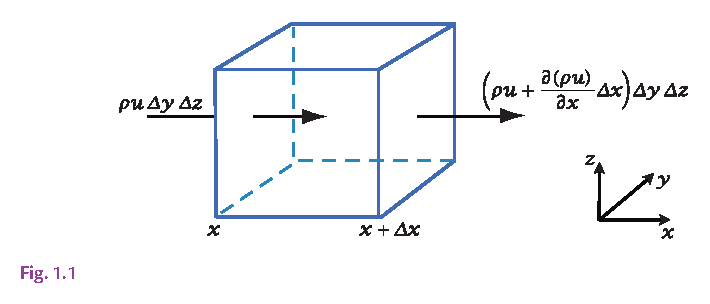
\includegraphics[width=0.7\textwidth]{assets/fig_continuity1.pdf}
  \caption{
    Mass conservation in an rectangular Eulerian control volume.
    The mass convergence, $\partial(\rho u)/\partial x$
    (plus contributions in the $y$ and $z$ directions),
    must be balanced by a density decrease.
    This is Fig. 1.1 in AOFD (Vallis, 2017).
  }
\end{figure}

\begin{figure}[h]
  \centering
  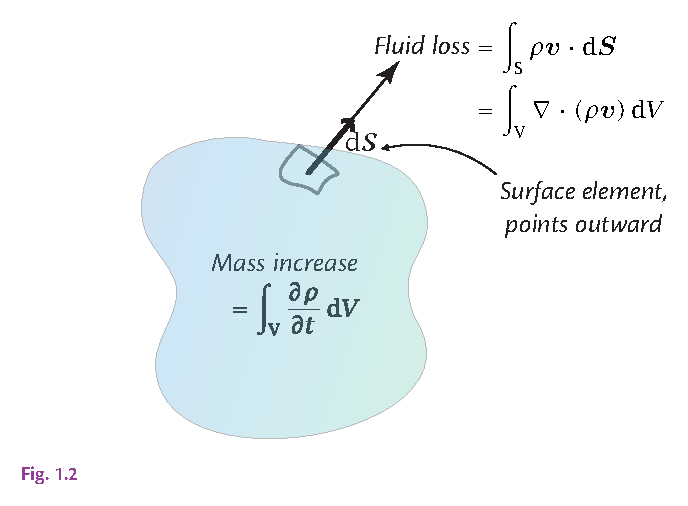
\includegraphics[width=0.7\textwidth]{assets/fig_continuity2.pdf}
  \caption{
    Mass conservation in an arbitrary Eulerian control volume $V$ bounded by a
    surface $S$. The mass increase, $\int_V(\partial \rho/\partial t)dV$
    is equal to the mass flowing into the volume,
    $-\int_S(\rho\mathbf{v}) \cdot d\mathbf{S} = -\int_V \nabla \cdot (\rho\mathbf{v})dV$.
    This is Fig. 1.2 in AOFD (Vallis, 2017).
  }
\end{figure}

\subsection{Conservation of momentum}

\subsection{Conservation of energy}

%\newpage
%\section{Rotating and stratified flows}

%\newpage
%\section{Shallow water equations}

%\newpage
%\section{Boundary layers}

%\newpage
%\section{Turbulence}

%\newpage
%\section{Surface gravity waves}


\printindex

\end{document}
